\documentclass[border=15pt]{standalone}
\usepackage{tikz}
\usepackage{tikz-3dplot}
\usetikzlibrary{positioning, 3d, shapes.geometric, arrows.meta, calc}

% Colors
\definecolor{InputColor}{RGB}{200,200,200}
\definecolor{StemColor}{RGB}{255,235,59}
\definecolor{ConvColor}{RGB}{255,193,7}
\definecolor{PoolColor}{RGB}{255,152,0}
\definecolor{TokenColor}{RGB}{156,39,176}

\begin{document}
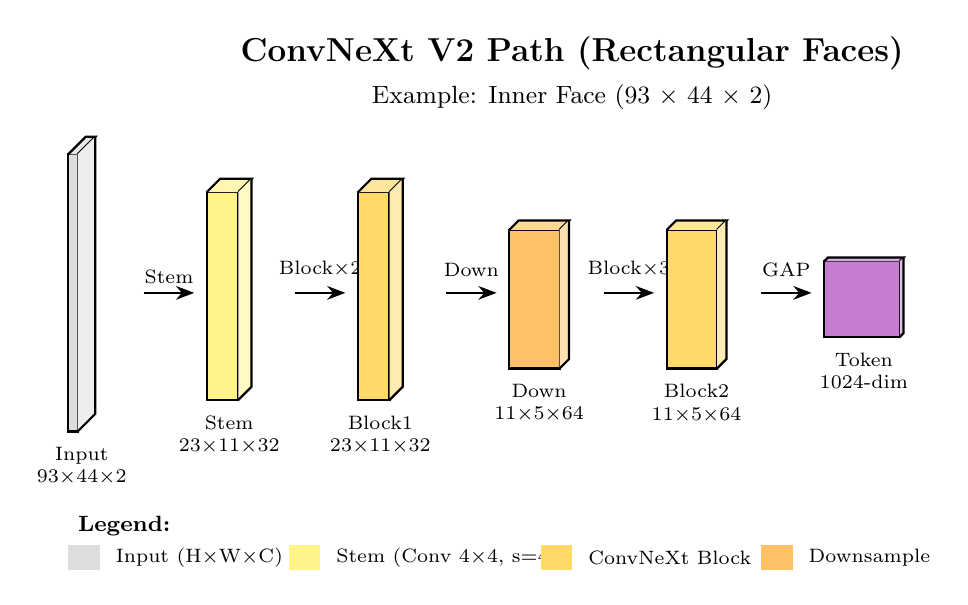
\begin{tikzpicture}[
    scale=0.8,
    every node/.style={font=\small},
    >=Stealth,
]

% Helper for 3D boxes (front face + depth lines)
% #1=x, #2=y, #3=width, #4=height, #5=depth, #6=color, #7=label
\newcommand{\featuremap}[7]{
    % Front face
    \fill[#6!60] (#1,#2) rectangle (#1+#3,#2+#4);
    \draw[thick] (#1,#2) rectangle (#1+#3,#2+#4);
    % Top face (parallelogram)
    \fill[#6!40] (#1,#2+#4) -- (#1+#5*0.3,#2+#4+#5*0.3) -- (#1+#3+#5*0.3,#2+#4+#5*0.3) -- (#1+#3,#2+#4) -- cycle;
    \draw[thick] (#1,#2+#4) -- (#1+#5*0.3,#2+#4+#5*0.3) -- (#1+#3+#5*0.3,#2+#4+#5*0.3) -- (#1+#3,#2+#4);
    % Right face (parallelogram)
    \fill[#6!30] (#1+#3,#2) -- (#1+#3+#5*0.3,#2+#5*0.3) -- (#1+#3+#5*0.3,#2+#4+#5*0.3) -- (#1+#3,#2+#4) -- cycle;
    \draw[thick] (#1+#3,#2) -- (#1+#3+#5*0.3,#2+#5*0.3) -- (#1+#3+#5*0.3,#2+#4+#5*0.3);
    % Label below
    \node[below, font=\scriptsize, align=center] at (#1+#3/2+#5*0.15, #2-0.1) {#7};
}

% Title
\node[font=\large\bfseries] at (8, 6) {ConvNeXt V2 Path (Rectangular Faces)};
\node[font=\small] at (8, 5.3) {Example: Inner Face (93 $\times$ 44 $\times$ 2)};

% Input: 93 x 44 x 2
\featuremap{0}{0}{0.15}{4.4}{0.93}{InputColor}{Input\\93$\times$44$\times$2}

% Arrow
\draw[->, thick] (1.2, 2.2) -- (2.0, 2.2);
\node[above, font=\scriptsize] at (1.6, 2.2) {Stem};

% After Stem: 23 x 11 x 32  (stride 4)
\featuremap{2.2}{0.5}{0.5}{3.3}{0.7}{StemColor}{Stem\\23$\times$11$\times$32}

% Arrow
\draw[->, thick] (3.6, 2.2) -- (4.4, 2.2);
\node[above, font=\scriptsize] at (4.0, 2.3) {Block$\times$2};

% After Block1: 23 x 11 x 32
\featuremap{4.6}{0.5}{0.5}{3.3}{0.7}{ConvColor}{Block1\\23$\times$11$\times$32}

% Arrow
\draw[->, thick] (6.0, 2.2) -- (6.8, 2.2);
\node[above, font=\scriptsize] at (6.4, 2.3) {Down};

% After Downsample: 11 x 5 x 64  (stride 2)
\featuremap{7.0}{1.0}{0.8}{2.2}{0.5}{PoolColor}{Down\\11$\times$5$\times$64}

% Arrow
\draw[->, thick] (8.5, 2.2) -- (9.3, 2.2);
\node[above, font=\scriptsize] at (8.9, 2.3) {Block$\times$3};

% After Block2: 11 x 5 x 64
\featuremap{9.5}{1.0}{0.8}{2.2}{0.5}{ConvColor}{Block2\\11$\times$5$\times$64}

% Arrow
\draw[->, thick] (11.0, 2.2) -- (11.8, 2.2);
\node[above, font=\scriptsize] at (11.4, 2.3) {GAP};

% Token: 1 x 1 x 1024
\featuremap{12.0}{1.5}{1.2}{1.2}{0.2}{TokenColor}{Token\\1024-dim}

% Legend
\node[font=\footnotesize\bfseries, anchor=west] at (0, -1.5) {Legend:};
\fill[InputColor!60] (0, -2.2) rectangle (0.5, -1.8); \node[anchor=west, font=\scriptsize] at (0.6, -2.0) {Input (H$\times$W$\times$C)};
\fill[StemColor!60] (3.5, -2.2) rectangle (4.0, -1.8); \node[anchor=west, font=\scriptsize] at (4.1, -2.0) {Stem (Conv 4$\times$4, s=4)};
\fill[ConvColor!60] (7.5, -2.2) rectangle (8.0, -1.8); \node[anchor=west, font=\scriptsize] at (8.1, -2.0) {ConvNeXt Block};
\fill[PoolColor!60] (11, -2.2) rectangle (11.5, -1.8); \node[anchor=west, font=\scriptsize] at (11.6, -2.0) {Downsample};

\end{tikzpicture}
\end{document}
